\cfoot{}\rhead{\thepage}
\lhead{{\scshape Work in progress} $\qquad$ {\tiny \today } }

% \noindent{\Large{\scshape\bfseries Entreé to Generic Extensions and Forcing in Set Theory}} \\[0.1cm]
%
% \noindent {\scshape Bohuslav Balcar}, {\small CTS, J{\' \i}lsk{\' a} 1, Praha 1,
% 	Czech Republic, {\ttfamily balcar@cts.cuni.cz} } \\[0.1cm]
% \noindent {\scshape Jonathan Verner}, {\small KTIML MFF UK, {\ttfamily jonathan.verner@matfyz.cz}\\[0.1cm]
% {\tiny \today } \\[0.5cm]

%\maketitle

\thispagestyle{empty}

%%%%%%%%%%%%%%%%%%%%%%%%%%%%%%%%%%%%%%%%%%%%%%%%%%%%%%%%%%%%%%%%%%%%%%%%%%%
%%%%%%%%%%%%%%%%%%%%%%%%%%%%%%%%%%%%%%%%%%%%%%%%%%%%%%%%%%%%%%%%%%%%%%%%%%%
\section{Work in progress}\label{work-in-progress}
\subparagraph{Reading of names} Given a forcing notion $(P,\leq)$ we have worked with different
relations $r\subseteq P\times V$ and when we had a generic filter $G$ on $P$ over $V$ we
considered semisets of the form $r[G]$. It is natural to look at the relation $r$ as an
approximation of this semiset. This approximation is a set from the groundmodel, in our case $V$.
The generic filter then `interprets' or `specifies' the exact meaning of $r$. In view of this,
we consider the relations to be `names' for semiset. We shall adopt the convention to `dot'
the relations, i.e. write $\dot{r}$ instead of $r$, when we want to emphasize that we are thinking
of them as names. We shall also write $\dot{r}/_G$ instead of $r[G]$.

Given a groundmodel set $x\in V$, we shall sometimes want to have a name for $x$, customarily
denoted by $\check{x}$. We could either choose $\check{x}$ to be some canonical relation
$\subseteq P\times x$ or, as we shall do here, we identify $\check{x}$ with $x$ and define
$\check{x}/_G$ to be $x$.

\subparagraph{Boolean names} \label{first-translation}
We have already mentioned, that the difference between an ordering $P$ and the complete Boolean
algebra $RO(P)$ is irrelevant from the point of view of forcing. However, working with a Boolean
algebra can sometimes be more convenient, since we can use the Boolean operations. We shall now
describe how to pass from $P$-names, i.e. relations $r\subseteq P\times V$, to appropriate
$B$-names (see also \ref{lost-in-translation}).

Starting with a name $r\subseteq P\times V$ we can consider the following modifications
$$\tilde{r} = \{\langle q,x\rangle:(\exists p\geq q)(\langle p,x\rangle\in r)\}$$
and
$$
\mathring{r} = \{\langle p,x\rangle: x\in rng(r)\ \&\ \{q\in P:\langle q,x\rangle\in\tilde{r}\}\ \mbox{is dense below}\ p\}.
$$
We immediately see that $dom(\tilde{r})=\bigcup\{(\leftarrow,p]:p\in dom(r)\}$ so $dom(\tilde{r})$
is downwards closed and $\tilde{r}[\{q\}] = \bigcup\{ r[\{p\}]:q\leq p\}$. Also, recalling
that a set $E\subseteq P$ is predense below $p\in P$ if there is no $q\leq p$ which would
be disjoint from $E$, i.e. $q\in E^\perp$, we see that $\langle p,x\rangle\in\mathring{r}$
iff $r^{-1}[\{x\}]$ is predense below $p$.

\begin{fact} It is clear that $r\subseteq\tilde{r}\subseteq\mathring{r}$ and, moreover,
\begin{itemize}
 \item[(i)] $\mathring{r}^{-1}[\{x\}]$ is a regular subset of $P$ for all $x$ (see \ref{Regularisation}).
 \item[(ii)] For any generic filter $G$ on $P$, the interpretations are the same, i.e. $r[G]=\tilde{r}[G]=\mathring{r}[G]$.
\end{itemize}
\end{fact}

The proof is straightforward. Note that in (ii) genericity of the filter $G$ is only needed for the last equality,
the first holds for any filter.


Using (i) and the fact that regular subsets of $P$ form a complete Boolean algebra denoted $RO(P)$ (see \ref{RO})
a relation $r\subseteq P\times V$ naturally determines a function $f:rng(r)\to RO(P)^+$, namely:
$$
f(x)=\mathring{r}^{-1}[\{x\}].
$$
For this function we have that for any generic filter $G$ on $P$
$$
r[G]=\{x:f(x)\in \bar{G}\},
$$
where $\bar{G}=\{x\in RO(P)^+: x\cap g\neq\emptyset\}$.

\subparagraph{Relationship between names and conditions}
We shall now introduce a piece of standard notation (see \ref{forcing-relation} for more details):
Given a name $\dot{r}\subseteq P\times V$, $x\in V$ and a condition $p\in P$ we shall write
$$
p\force x\in\dot{r}\ \mbox{or, more precisely}\ p\force\check{x}\in\dot{r}
$$
iff $\langle p,x\rangle\in\mathring{r}$. It is said that `the condition $p$ knows that $x$ is an element of $\dot{r}$'
or `p forces $\check{x}\in\dot{r}$.'.

What about $p$ forcing that $x$ is \emph{not} in $\dot{r}$. We might be tempted to that
$p\force \check{x}\not\in\dot{r}$ means $\langle p,x\rangle\not\in\mathring{r}$.
It turns out, however, that this would not work in general because $\langle p,x\rangle\not\in\mathring{r}$ might
mean that $p$ just doesn't know whether $\check{x}\in\dot{r}$. The correct definition
will be
$$p\force\check{x}\not\in\dot{r}\ \mbox{iff}\ p\ \mbox{is disjoint from all elements of}\ r^{-1}[\{x\}],$$
i.e. $p\in \{q\in P:q\force\check{x}\in\dot{r}\}^\perp$.

So in general, given a condition $p\in P$, a name $\dot{r}$ and an element $x\in V$ there are three possibilities:
\begin{itemize}
 \item[(i)]   $p\force\check{x}\in\dot{r}$
 \item[(ii)]  $p\force\check{x}\not\in\dot{r}$
 \item[(iii)] $p$ does not know, i.e. there are (disjoint) elements $q_1,q_2\leq p$ such
              that $q_1\force\check{x}\in\dot{r}$ and $q_2\force\check{x}\not\in\dot{r}$.
\end{itemize}

The generic filter $G$ allows us to evade three valued or even intuitionistic logic since whenever
$p\in P\cap G$ such that $p$ does not decide $\check{x}\in\dot{r}$ the set
$$
H=\{ q\leq p:q\force\check{x}\in\dot{r}\ \vee\ q\force\check{x}\not\in\dot{r}\}
$$
is open dense below $p$ so there is $q\in G\cap H$ below $p$ which decides $\check{x}\in\dot{r}$.

\subparagraph{The role of dense subsets}
Consider a forcing notion $P$ with a dense subset $H\subseteq P$. In the previous chapter we have said that it does not matter
whether we work with $P$ or $H$. However, given a $P$-name $\dot{r}$ it is not immediately clear that this is an $H$-name.
In fact, it need not be, since, e.g. $dom(r)\cap H$ can be empty. To overcome this, we pass to $\tilde{r}$ for which we
necessarily have $dom(\tilde{r})\cap H\neq\emptyset$ (provided $dom(r)$ was nonempty). Moreover it turns out that for
each $h\in H$, $x\in V$ we have
$$
h\force\check{x}\in\dot{r}\ \mbox{iff}\ h\force\check{x}\in\tilde{r}
$$
An easy density argument now shows that $\dot{r}$ and $\dot{s}=\tilde{r}\cap H\times\dom(r)$ are names for the same semiset,
i.e. $\dot{r}/_G = \dot{s}/_G$ for each generic filter $G$.

\subparagraph{Equality of names}
When we will be trying to prove the consistency of the failure of CH, we will do this by adding semisets which are subsets of $\omega$.
For this to work we have to add a lot of different semisets, however we only have names for the semisets and we know, that different
names can be actually names for the same semiset. So it will be important to know, when two names are really names for different semisets.
We first start with the opposite question: When are two names $\dot{r}$ and $\dot{s}$ names for the same semiset?
The answer is that a condition $p\in P$ `knows' that the two $P$-names $\dot{r},\dot{s}$ are actually equal, i.e. $\dot{r}/_G=\dot{s}/_G$ for any generic $G$ containing $p$, iff for any $x\in rng(r)\cup rng(s)$ one of the following equivalent conditions is met:
\begin{itemize}
 \item[(i)]  $(\forall q\leq p)(r^{-1}[\{x\}]\ \mbox{is predense below}\ q\ \leftrightarrow s^{-1}[\{x\}]\ \mbox{is predense below}\ q)$
 \item[(ii)] $(\forall q\leq p)(q\perp r^{-1}[\{x\}]\leftrightarrow q\perp s^{-1}[\{x\}])$
\end{itemize}
If one of these conditions is met, we write $p\force\dot{r}=\dot{s}$ and we write $P\force\dot{r}=\dot{s}$ if all conditions
force $\dot{r}$ and $\dot{s}$ to be equal, i.e. iff $(\forall x\in dom(r)\cup dom(s) )((r^{-1}[\{x\}])^\perp = (s^{-1}[\{x\}])^\perp)$. This
implies that, necessarily, $rng(r)=rng(s)$.


{\bf Examples}

{\bf (i)} We say that $P$ forces $\check{x}\in\dot{r}$ if each $p\in P$ forces $\check{x}\in\dot{r}$. Clearly
$P\force\check{x}\in\dot{r}$ iff $r^{-1}[\{x\}]$ is predense in $P$ and $P\force\check{x}\not\in\dot{r}$ iff
$r^{-1}[\{x\}]=\emptyset$.

{\bf (ii)} Given two names $\dot{r},\dot{s}$ then
\begin{itemize}
 \item[(a)] $p\force\dot{r}=\dot{s}$ iff $(forall x\in rng(r)\cup rng(s))(\forall q\leq p)(q\force \check{x}\in\dot{r} \leftrightarrow q\force\check{x}\in\dot{s})$
 \item[(b)] $p\not\force\dot{r}=\dot{s}$ iff $(\exists q\leq p)(\exists x)(q\force\check{x}\in\dot{r}\ \&\ q\force\check{x}\not\in\dot{s}\ \vee\
                                                                           q\force\check{x}\in\dot{s}\ \&\ q\force\check{x}\not\in\dot{r})$
 \item[(c)] $p\force\dot{r}\neq\dot{s}$ iff $(\forall p_1\leq p)(\exists q\leq p_1)(q\not\force\dot{r}=\dot{s})$
\end{itemize}

{\bf (iii)}
\begin{itemize}
 \item[(a)] $P\force \dot{r}\subseteq\check{\omega}$ iff $rng(r)\subseteq\omega$
 \item[(b)] $p\force \dot{r}\subseteq\check{\omega}\ \&\ \dot{r}\ \mbox{is infinite}$ iff $rng(r)\subseteq\omega$ and
            $(\forall m<\omega)(p\force(\exists \dot{n})(\check{m}\leq \dot{n}\ \&\ \dot{n}\in\dot{r}))$ iff for all $m<\omega$ the set
            $r^{-1}[(\omega\setminus m)]$ is predense below $p$ iff for any generic filter $G$ with $p\in G$ the semiset $\dot{r}/_G$ is an
            infinite part of $\omega$.
 \item[(c)] $p\force\dot{r}\subseteq\check{\omega}\ \&\ \dot{r}\ \mbox{is finite}$ iff $rng(r)\subseteq\omega$ and
            $(\forall p_1\leq p)(\exists q\leq p_1)(\exists k<\omega)(q\in (r^{-1}[(\omega\setminus k)])^\perp)$.
\end{itemize}
{\bf (iv)} $P\force\dot{r}:\check{\omega}\to\check{\omega}$, i.e. $P$ forces that $\dot{r}$ is a mapping of $\omega$ into $\omega$ iff
           for each $p\in P$ the set
           $$
             r^\heartsuit(p) = \bigcup r[\ [p,\rightarrow)\ ]
           $$
           is a mapping of $P$ into partial functions from $\omega$ into $\omega$ and for any $n\in\omega$ the set
           $$
             \{p\in P:n\in dom(r^\heartsuit(p))\}
           $$
           is dense in $P$.

           Now suppose $B=RO(P)$ and $P\force \dot{r}:\check{\omega}\to\check{\omega}$. Then the name $\dot{r}$ determines an $(\omega,\omega)$-matrix
           on $B$ as follows:
           $$
           a(n,m)=\bigvee\{p\in P:\langle n,m\rangle\in r^\heartsuit(p)\}.
           $$


%\newcommand{\norm}[1]{\parallel #1\parallel}
%\newcommand{\R}{\mbox{${\Bbb R}$}}
%\newcommand{\N}{\mbox{${\mathcal N}$}}
\newcommand{\M}{\mbox{${\mathcal M}$}}
\newcommand{\A}{\mbox{${\mathcal A}$}}
\newcommand{\U}{\mbox{${\mathcal U}$}}

\subsection{Cicho\'n's diagram and cardinal characteristics}

This section will be devoted to an introduction to topic of cardinal characteristics of the continuum. Most of
these cardinal numbers are associated with some properties of the real line. They are all greater or equal
to $\omega_1$ and less or equal to $\cont$, but in general their value is not decided by the usual axioms of ZFC.
Positing that some cardinal invariant is equal to $\cont$ may be seen as a weakening of the continuum hypothesis
and in fact many constructions which work under CH may be carried out under weaker assumptions of this form.
For a beautiful exposition of the topic see \cite{Bl:2009}.

We start with the following general definition, which will be used mainly in the case that the ideal
$I$ is either the ideal of meager sets of $\R$ (denoted $\M$) or the ideal sets having \emph{Lebesgue measure zero}
(denoted by $\N$).

\begin{definition} For any ideal ${\mathcal I}$ on a set $X$ we define the following cardinal characteristics:
 \begin{eqnarray*}
  \hbox{add}({\mathcal I})  &=& min\{|{\mathcal A}|:{\mathcal A}\subseteq {\mathcal I}\ \&\ \bigcup{\mathcal A} \not\in I\}\cr
  \hbox{non}({\mathcal I}) &=& min\{|A|:A\subseteq X\ \&\ A\not\in {\mathcal I}\}\cr
  \hbox{cov}({\mathcal I})  &=& min\{|{\mathcal A}|:{\mathcal A}\subseteq {\mathcal I}\ \&\ \bigcup{\mathcal A} = \bigcup{\mathcal I}\}\cr
  \hbox{cof}({\mathcal I})  &=& min\{|{\mathcal A}|:{\mathcal A}\subseteq {\mathcal I}\ \&\ (\forall I\in{\mathcal I})(\exists A\in{\mathcal A})(I\subseteq A)\}\cr
 \end{eqnarray*}
\end{definition}
The following is a summary definition of some of the important cardinal characteristics:
\begin{definition}
 We define the following cardinals
 \begin{eqnarray*}
  {\mathfrak b} &=& min\{|\A|:\A\subseteq {}^\omega\omega\ \&\ (\forall f\in{}^\omega\omega)(\exists g\in\A)(g\not\leq^* f)\}\cr
  {\mathfrak d} &=& min\{|\A|:\A\subseteq {}^\omega\omega\ \&\ (\forall f\in{}^\omega\omega)(\exists g\in\A)(f\leq^* g)\}\cr
  {\mathfrak a} &=& min\{|\A|:\A\subseteq [\omega]^\omega\ \&\ \omega\leq|\A|\ \& (\forall B\in[\omega]^\omega)(\exists A\in\A)(|A\cap B|=\omega)\}\cr
  {\mathfrak s} &=& min\{|\A|:\A\subseteq [\omega]^\omega\ \& (\forall B\in[\omega]^\omega)(\exists A\in\A)(|A\cap B|=|(\omega\setminus A)\cap B|=\omega)\}\cr
  {\mathfrak u} &=& min\{|\U|:\U\subseteq [\omega]^\omega\ \&\ \omega\leq|\A|\ \& (\forall B\in[\omega]^\omega)(\exists A\in\U)(|A\cap B|<\omega\vee A\subseteq^* B))\}\cr
  {\mathfrak h} &=& min\{\kappa:\pw(\omega)/FIN\ \hbox{is not}\ (\kappa,\cdot,2)\hbox{-distributive}\}\cr
  {\mathfrak p} &=& min\{|\U|:\U\subseteq [\omega]^\omega\ \&\ (\forall {\mathcal V}\in[\U]^{<\omega})(|\bigcap {\mathcal V}|=\omega)\ \&\ (\forall P\in[\omega]^\omega)(\exists U\in\U)(P\not\subseteq^* U)\}\cr
  {\mathfrak t} &=& min\{|\U|:\U\subseteq [\omega]^\omega\ \&\ \U\ \hbox{is linearly ordered by}\ \subseteq^*\ \&\ (\forall P\in[\omega]^\omega)(\exists U\in\U)(P\not\subseteq^* U)\}\cr
  {\mathfrak i} &=& min\{|\A|:\A\subseteq [\omega]^\omega\ \&\ \A\ \hbox{is independent}\ \&\ (\forall \A^\prime\subseteq[\omega]^\omega)(\A^\prime\subseteq\A\rightarrow\A^\prime\ \hbox{is not independent})\}\cr
  {\mathfrak m} &=& min\{\kappa:MA_\kappa\ \hbox{fails}\}
 \end{eqnarray*}
\end{definition}

\begin{definition}A family ${\mathcal G}\subseteq[\omega]^\omega$ is \emph{groupwise dense} if it is closed under almost subsets and for any infinite partition of $\omega$ into intervals there are infinitely many intervals from the partition whose union is in ${\mathcal G}$. The \emph{groupwise density number} ${\mathfrak g}$ is now
defined to be the smallest cardinality of a set $\A$ of groupwise dense families with $\bigcap\A=\emptyset$.
\end{definition}

It turns out that it is very usefull to think of these definitions in the following way (introduced and isolated explicitly in \cite{Voj:93}, but
implicitly appearing already in \cite{Fre:84} and in an unpublished work of Miller).

\begin{definition} Suppose we are given a triple ${\mathbf A}=(A_-,A_+,R)$ consisting of a set $A_-$ of challenges a set $A_+$ of responses and
a relation $R\subseteq A_-\times A_+$. We say that $b\in A_+$ is a response to a challenge $a\in A_-$ iff $aRb$.
We define the \emph{norm} $||{\mathbf A}||=||(A_-,A_+,R)||$ of this triple to be:
\begin{displaymath}
 ||(A_-,A_+,R)||=\min\{|{\mathcal B}|:{\mathcal B}\subseteq A_+\ \&\ (\forall a\in A_-)(\exists b\in{\mathcal B})(aRb)\}.
\end{displaymath}
In other words the norm is the cardinality of the smallest set of responses which are enough to answer every challenge. We also
define the \emph{dual} ${\mathbf A}^\perp$ of ${\mathbf A}$ to be the triple $(A_+,A_,-(R^{-1}))$, where $(x,y)\in -(R^{-1})\equiv (y,x)\not\in R$.
\end{definition}

Note that most of the cardinal invariants considered so far are norms of some triple. The usefulness of this framework lies in the fact
that the notion of duality gives a precise meaning to the intuition that some of the cardinals defined (e.g. $\mathfrak b,d$) are very
intimately connected to each other.

The definition of a Tukey connection (which is a morphism between triples in the sense of category theory)

\begin{definition}[Tukey's connection] Given two ordering triples ${\mathbf A}=(A_-,A_+,R), {\mathbf B}=(B_-, B_+, Q)$ we say that ${\mathbf A}\geq_T {\mathbf B}$ if there are functions $\phi_-:B_-\to A_-$ and $\phi_+:A_+\to B_+$ which satisfy:
\begin{displaymath}
 (\forall b\in B_-, a\in A_+)(\phi_-(b)Ra\rightarrow b Q\phi_+(a))
\end{displaymath}
Following Blass we call the pair $\phi=(\phi_-,\phi_+)$ a \emph{morphism} from $\mathbf A$ to $\mathbf B$ (Vojtáš calls $\phi$ a generalized Galois-Tukey connection from $\mathbf B$ to $\mathbf A$) and we shall write $\phi:{\mathbf A}\to {\mathbf B}$. Note that if $\phi:\mathbf A\to \mathbf B$ then $\phi^\perp=(\phi_+,\phi_-)$ is
a morphism from ${\mathbf B}\perp$ to ${\mathbf A}^\perp$.
\end{definition}

It is instructive to think of $\mathbf A\geq_T \mathbf B$ as saying that meeting challenges in $\mathbf B$ is not harder then meeting challenges in $\mathbf A$,
(cf. the notion of a Borel reduction of two Borel Equivalence relations or the notion of Turing reducibility in Recursion theory).

\begin{obs} If ${\mathbf A}\leq_T{\mathbf B}$ then $\norm{{\mathbf A}}\leq_T\norm{{\mathbf B}}$.
\end{obs}

The following diagram (see \cite{Fre:84}) summarizes all that can be proved in ZFC concerning the relations between cardinal invariants defined
from the ideal of null and meager sets:

\begin{theorem}[Cincho\'n's diagram]
%\begin{displaymath}
%\begin{array}{ccccccc}
%
%\hbox{cov}({\mathcal N}) &\longrightarrow & \hbox{non}({\mathcal M}) &\longrightarrow &\hbox{cof}({\mathcal M})  &\longrightarrow & \hbox{cof}({\mathcal N})  \cr
%                         &                & \uparrow                  &                &\uparrow                  &                &                           \cr
%\uparrow                 &                & {\mathfrak b}             &\longrightarrow &{\mathfrak d}             &                &\uparrow                   \cr
%                         &                & \uparrow                  &                &\uparrow                  &                &                           \cr
%\hbox{add}({\mathcal N}) &\longrightarrow & \hbox{add}({\mathcal M})  &\longrightarrow &\hbox{cov}({\mathcal M})  &\longrightarrow & \hbox{non}({\mathcal N}) \cr
%\end{array}
%\end{displaymath}
\end{theorem}
\begin{center}
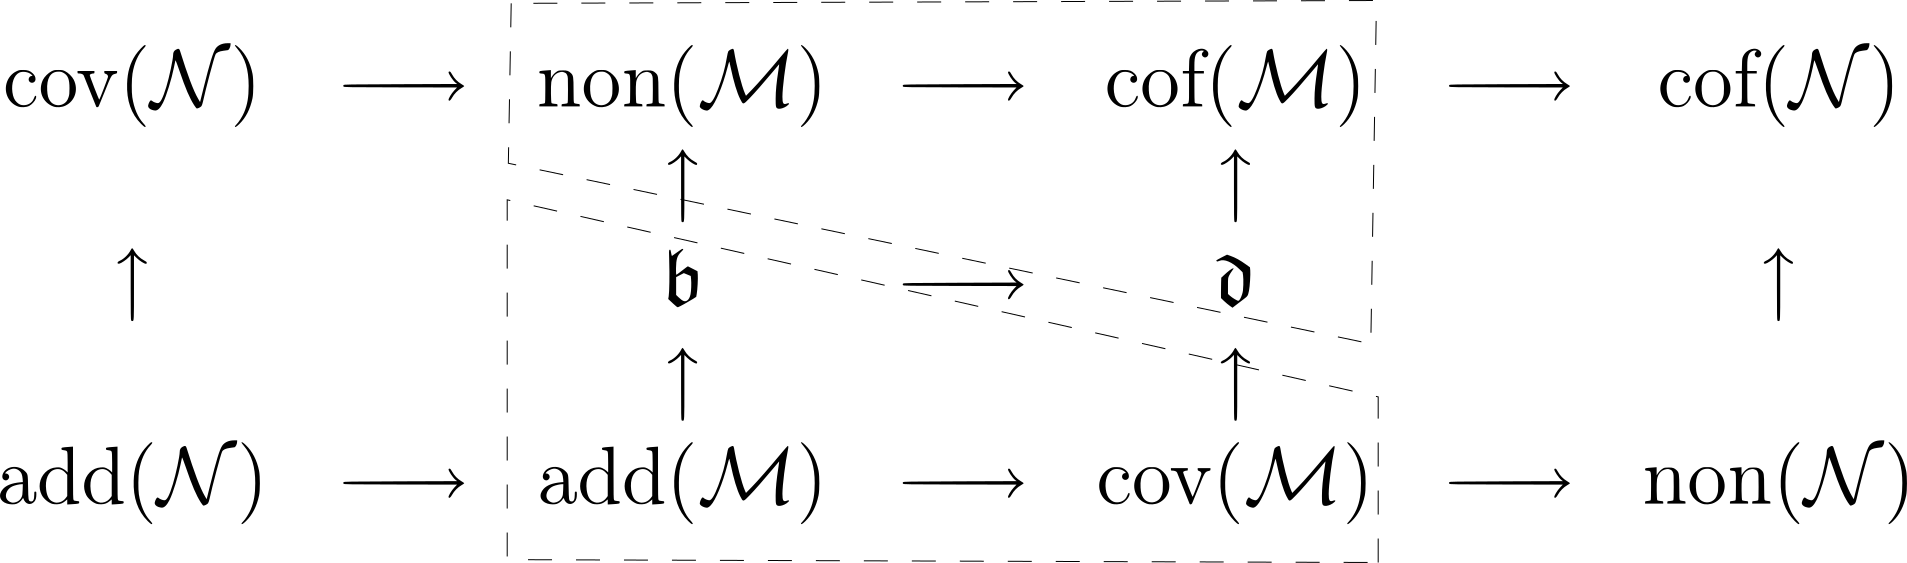
\includegraphics[height=3cm]{work_in_progress/cichon-2.pdf}
\end{center}

It is a direct consequence of the following reformulation of the cardinal invariants in terms of norms of triples:

\begin{theorem}
 \begin{displaymath}
\begin{array}{ccccccc}

(\R,\N,\in)        &\longrightarrow & (\M,\R,\not\ni)                         &\longrightarrow & (\M,\M,\subset)                    & \longrightarrow &(\N,\N,\subset)\cr
                   &                & \uparrow                                &                &\uparrow                            &                 &               \cr
\uparrow           &                & (\omega^\omega,\omega^\omega,\not\geq^*)&\longrightarrow &(\omega^\omega,\omega^\omega,\leq^*)&                 &\uparrow       \cr
                   &                & \uparrow                                &                &\uparrow                            &                 &               \cr
(\N,\N,\not\supset)&\longrightarrow & (\M,\M,\not\supset)                     &\longrightarrow &(\R,\M,\in)                         & \longrightarrow &(\N,\R,\not\ni)\cr
\end{array}
\end{displaymath}
\end{theorem}

A summary of the connections between different cardinal invariants can be seen in the following diagram. It is a fusion of
Cicho\'n's diagram with van Douwen's diagram which can be found in \cite{Bl:2009} (see also \cite{Br:2006}):

\begin{center}
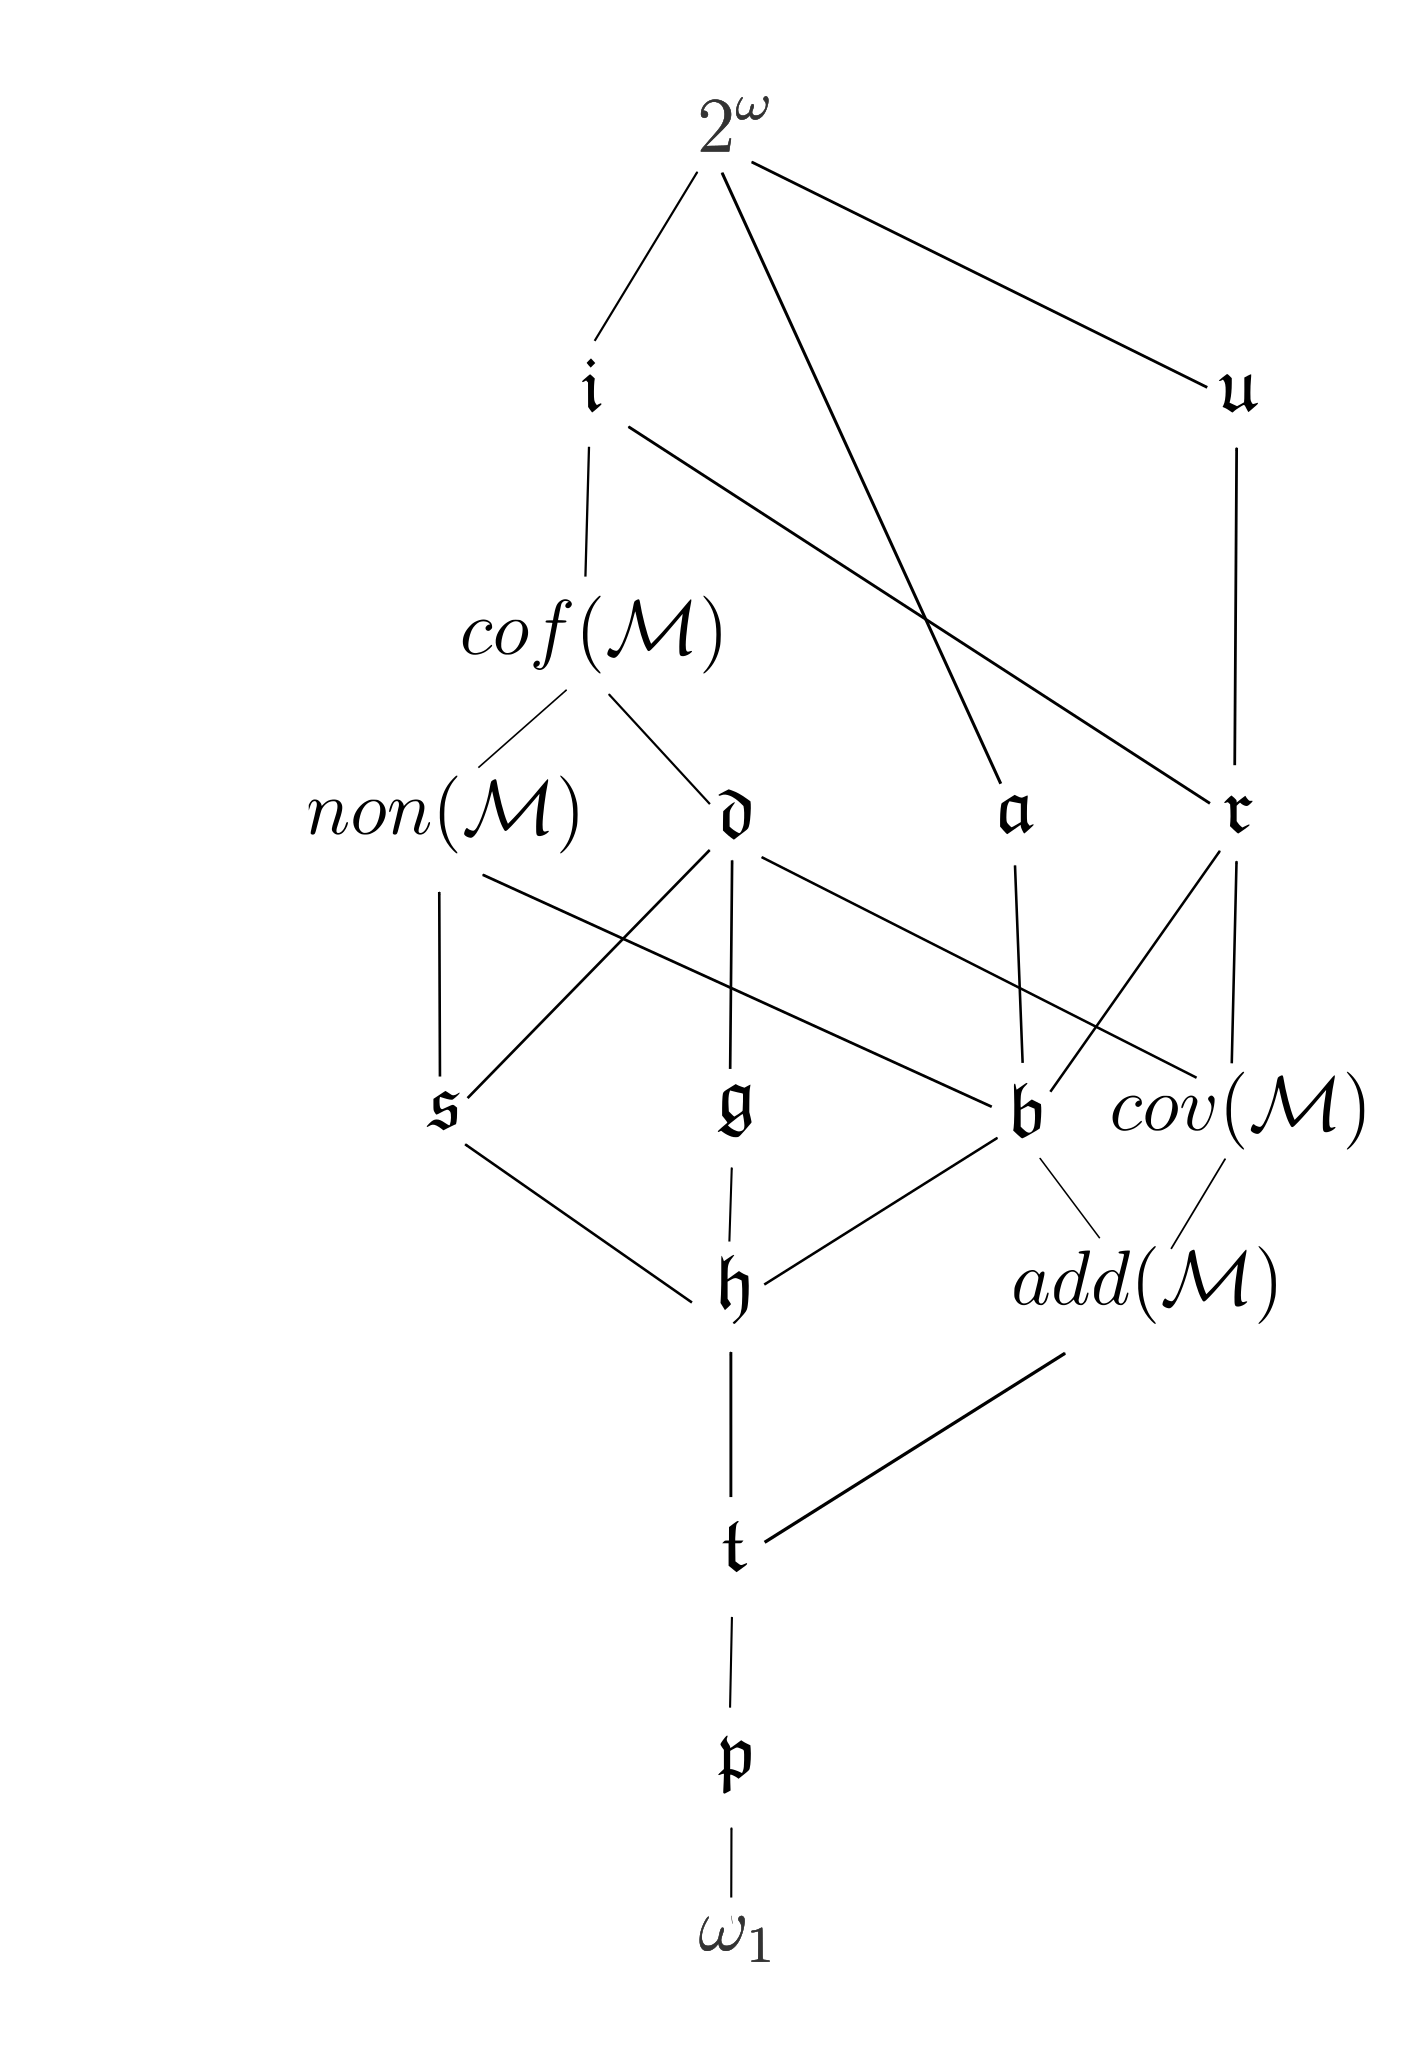
\includegraphics[height=10cm]{work_in_progress/cardinal-invariants-diagram-varIII.pdf}
\end{center}

The dashed boxes indicate, respectively, that the top cardinal and bottom cardinal are the maximum and the minimum of the other
two cardinals.
\subsection{iteration}

% \subsubsection{Martin's axiom}
%
% Take $\kappa$ s.t., $\kappa^{<\kappa}=\kappa$. Consider $\mathcal S=\{(P,\leq):P\subseteq \kappa, |P|<\kappa\}$ ordered by regular embedding.
% If $B$ is a generic on $S$ then forcing with $B$ gives us MA.


\subsubsection{Preservation theorems}
\begin{definition} An ordering $P$ is \emph{$n$-linked}, $n<\omega$, if for any $X\in[P]^{\leq n}$ there is
$p\in P$ compatible with each $x\in X$. \emph{Linked} is short for $2$-linked. An ordering has the \emph{Knaster} property if any uncountable subset of the ordering contains an uncountable linked subset.
\end{definition}

\begin{obs} If $P$ has the Knaster property then given $n<\omega$ any uncountable subset contains
 an uncountable $n$-linked subset.
\end{obs}
\begin{proof} Easy, inductively apply the Knaster property to the witnesses for $2$-linkedness.
\end{proof}

\begin{proposition} If $P$ is an ordering with the Knaster property and $P\force\dot{Q}$ has the Knaster
 property then $P*\dot{Q}$ has the Knaster property.
\end{proposition}
\begin{proof}
 Let $\{\langle p_\alpha,\dot{q}_\alpha\rangle:\alpha<\omega_1\}\subseteq P*\dot{Q}$.
 By strengthening the $p_\alpha$'s we may assume that each $p_\alpha$ decides the statement

 \begin{displaymath}
  \{\dot{q}_\alpha:\alpha< \omega_1\}\ \hbox{is uncountable}
 \end{displaymath}

 By the above observation we may assume that the $p_\alpha$'s are $4$-linked. We also assume that all the
 $p_\alpha$'s decide the statement in the same way. There are two cases:

 {\bf Case 1.} Each $p_\alpha$ forces that $\{\dot{q}_\alpha:\alpha<\omega_1\}$ is uncountable. Working
 in $RO(P)$ (which also has the Knaster property) let $b=\bigvee\{p_\alpha\}$. Then $b$ forces that
 $\{\dot{q}_\alpha:\alpha<\omega_1\}$ is uncountable and since $P\force\dot{Q}$ has the Knaster property,
 there is a name $\dot{X}$ such that
 \begin{displaymath}
  b\force \dot{X}\subseteq\{\dot{q}_\alpha:\alpha<\omega_1\}\ \&\ |\dot{X}|=\omega_1\ \&\ \dot{X}\
  \mbox{is linked}.
 \end{displaymath}
 By induction to $\omega_1$ choose
 $\{\langle r_\alpha,\dot{s}_\alpha\rangle :\alpha<\omega_1\}\subseteq
  \{\langle p_\beta,\dot{q}_\beta\rangle:\beta<\omega\}$
 such that $r_\alpha\force \dot{s}_{\alpha+1}\in\dot{X}$. This is possible since each $p_\alpha$
 forces $\dot{X}$ to be uncountable. We claim that
 $\{\langle r_{\alpha+1},\dot{s}_{\alpha+1}\rangle:\alpha<\omega_1\}$
 is linked. Choose $\alpha,\beta<\omega_1$. Since we assumed the $p_\alpha$'s are $4$-linked we may find
 $p\in P$ be below $r_\alpha,r_{\alpha+1},r_\beta,r_{\beta+1}$.
 Then $p\force \dot{s}_{\alpha+1},\dot{s}_{\beta+1}\in \dot{X}$ so $p$ knows they are compatible so there
 is $\dot{t}\in \dot{Q}$ such that $p\force \dot{t}\leq \dot{s}_{\alpha+1},\dot{s}_{\beta+1}$. Then
 $\langle p,\dot{t}\rangle\leq\langle r_{\alpha+1},\dot{s}_{\alpha+1}\rangle,\langle r_{\beta+1},dot{s}_{\beta+1}\rangle$ and this finishes the proof of case 1.

 {\bf Case 2.} There is $R=\{\dot{r}_n:n<\omega\}\subseteq\dot{Q}$ such that
 $\dot{p}_\alpha\force\dot{q}_\alpha\in R$. Again work in $RO(P)$ and find, below each $p_\alpha$
 an antichain $b_{\alpha,n}$ such that $b_{\alpha,n}=||\dot{q}_\alpha=\dot{r}_n||$.
 By the Knaster property for $RO(P)$ there is an uncountable set $I\subseteq\omega_1\times\omega$
 such that for each $(\alpha,n),(\beta,m)\in I$ the corresponding $b_{\alpha,n}$ and $b_{\beta,m}$
 are compatible. Since $I$ is uncountable we may assume that the second coordinates are all equal to
 some $n_0<\omega$ and then $b_{\alpha,n_0}\leq p_\alpha$ and $b_{\alpha,n_0}\force \dot{q}_\alpha=\dot{r}_n$
 so they witness that $\langle p_\alpha,\dot{q}_\alpha\rangle$ are pairwise compatible.

\end{proof}


%%%%%%%%%%%%%%%%%%%%%%%%%%%%%%%%%%%%%%%%%%%%%%%%%%%%%%%%%%%%%%%%%%%%%%%
%%%                          END                                    %%%
%%%%%%%%%%%%%%%%%%%%%%%%%%%%%%%%%%%%%%%%%%%%%%%%%%%%%%%%%%%%%%%%%%%%%%%